\chapter{The Paradigm Shift}
\label{ch:paradigm-shift}

\begin{quote}
\itshape
``We shape our tools, and thereafter our tools shape us.''\\
--- Marshall McLuhan
\end{quote}

\vspace{0.5cm}

\noindent
On November 30, 2022, OpenAI released ChatGPT to the public. Within five days, it had one million users. Within two months, it had one hundred million. No technology in history had been adopted this fast---not the internet, not the iPhone, not even TikTok. But the real revolution wasn't in the consumer product. It was in what the underlying technology implied for the practice of software engineering.

Large Language Models are not merely another tool in the engineer's toolkit, like a new framework or a faster database. They represent a fundamentally different kind of computational primitive: one that is probabilistic rather than deterministic, that learns from data rather than being explicitly programmed, and that can generate novel outputs rather than simply transforming inputs according to fixed rules. For software engineers---professionals whose entire discipline is built on determinism, reproducibility, and formal correctness---this is a paradigm shift of the first order.

This chapter sets the stage for the rest of the book by examining what has changed, what hasn't, and why software engineers are uniquely positioned to lead in this new era.

\section{Software Engineering Before and After LLMs}

For the past fifty years, software engineering has been built on a foundation of deterministic computation. Given the same inputs, a well-written program produces the same outputs. Tests pass or fail. Bugs are reproducible. Code reviews verify logic. Deployment pipelines enforce invariants. The entire apparatus of modern software engineering---continuous integration, type systems, formal verification, chaos engineering---exists to tame complexity and ensure predictable behavior.

LLMs upend this foundation. Consider a simple function call:

\begin{lstlisting}[language=Python, caption={A traditional function vs. an LLM call}]
# Deterministic: same input, same output, every time
def calculate_tax(income: float, rate: float) -> float:
    return income * rate

# Probabilistic: same input, potentially different output
def summarize_document(doc: str) -> str:
    return llm.generate(
        prompt=f"Summarize this document:\n{doc}",
        temperature=0.3
    )
\end{lstlisting}

The \code{calculate\_tax} function is everything a software engineer expects: pure, testable, and deterministic. The \code{summarize\_document} function is none of those things. Its output varies between calls. Its correctness is subjective. Its performance depends on a model that was trained on data you didn't curate, using an architecture you didn't design, running on infrastructure you don't control.

And yet, \code{summarize\_document} can do something that no amount of traditional programming can achieve: it can understand and generate natural language with remarkable fluency. It can translate between languages, write code, answer questions, and reason about novel situations. This capability is so valuable that the challenge of working with non-deterministic systems is not just worth accepting---it's worth \emph{mastering}.

\subsection{The Old World: Programs as Explicit Instructions}

In traditional software engineering, the relationship between intent and implementation is explicit. When a product manager says ``we need to detect spam,'' an engineer writes rules:

\begin{lstlisting}[language=Python, caption={Traditional rule-based spam detection}]
def is_spam(message: str) -> bool:
    spam_keywords = ["buy now", "free money", "act fast"]
    if any(kw in message.lower() for kw in spam_keywords):
        return True
    if count_links(message) > 5:
        return True
    if message.isupper() and len(message) > 100:
        return True
    return False
\end{lstlisting}

Every decision is visible in the code. The logic can be reviewed, debugged, and explained to a regulator. But the approach is fragile: spammers evolve faster than rules, and the function captures only a tiny slice of what humans intuitively recognize as spam.

\subsection{The New World: Programs as Learned Behaviors}

With LLMs, the same task looks fundamentally different:

\begin{lstlisting}[language=Python, caption={LLM-powered spam detection}]
def is_spam(message: str) -> bool:
    response = llm.generate(
        prompt=f"""Classify the following message as SPAM or NOT_SPAM.
        Consider: urgency language, suspicious links, impersonation,
        too-good-to-be-true offers, and social engineering patterns.
        
        Message: {message}
        
        Classification:""",
        temperature=0.0,
        max_tokens=10,
    )
    return "SPAM" in response.upper()
\end{lstlisting}

The logic is no longer in the code---it's in the model's weights, learned from billions of examples during training. The code is merely a thin orchestration layer. This inversion---from logic-in-code to logic-in-weights---is the fundamental shift that this book addresses.

\begin{keytakeaway}
The transition from deterministic to probabilistic programming doesn't eliminate the need for software engineering. It \emph{increases} it. Systems built on probabilistic components require more sophisticated testing, monitoring, evaluation, and failure handling than their deterministic counterparts.
\end{keytakeaway}

\section{Why Software Engineers Need to Understand LLMs}

There is a tempting narrative that software engineers can treat LLMs as black boxes---API endpoints that accept text and return text. Just call the API, parse the response, and ship the feature. This approach works for prototypes. It fails catastrophically in production.

Here is why:

\subsection{You Cannot Test What You Don't Understand}

Traditional software testing relies on the engineer's ability to enumerate edge cases based on their understanding of the system's logic. If you know the function uses integer division, you test with zero. If you know it parses dates, you test with leap years. But when the ``logic'' lives inside a neural network with hundreds of billions of parameters, what do you test?

Engineers who understand how LLMs work---how they process tokens, how attention mechanisms focus on relevant context, how the temperature parameter affects output distribution---can write meaningfully better tests. They know that LLMs struggle with precise counting, that they can be confused by adversarial inputs, that they perform differently on in-distribution vs. out-of-distribution data. This knowledge directly translates to better test coverage and fewer production incidents.

\subsection{You Cannot Optimize What You Don't Measure}

LLM inference is expensive. A single GPT-5.5 call can cost \$0.03 to \$0.12 depending on token count. At scale---millions of requests per day---this adds up to hundreds of thousands of dollars per month. Engineers who understand the relationship between context window size, KV-cache memory, and inference latency can make architectural decisions that reduce costs by 10x or more.

\subsection{You Cannot Debug What You Cannot Reason About}

When an LLM-powered feature produces incorrect output, the debugging process is fundamentally different from traditional software. You can't set a breakpoint in the model's forward pass. You can't inspect individual neuron activations in production. But you \emph{can} reason about the problem if you understand the training data, the model's capabilities and limitations, and the prompt's role in steering behavior.

\section{The New Software Stack}

The emergence of LLMs has created a new layer in the software stack that sits between traditional application logic and the user experience. We call this the \term{AI orchestration layer}---the set of components responsible for managing interactions with language models.

\begin{figure}[htbp]
\centering
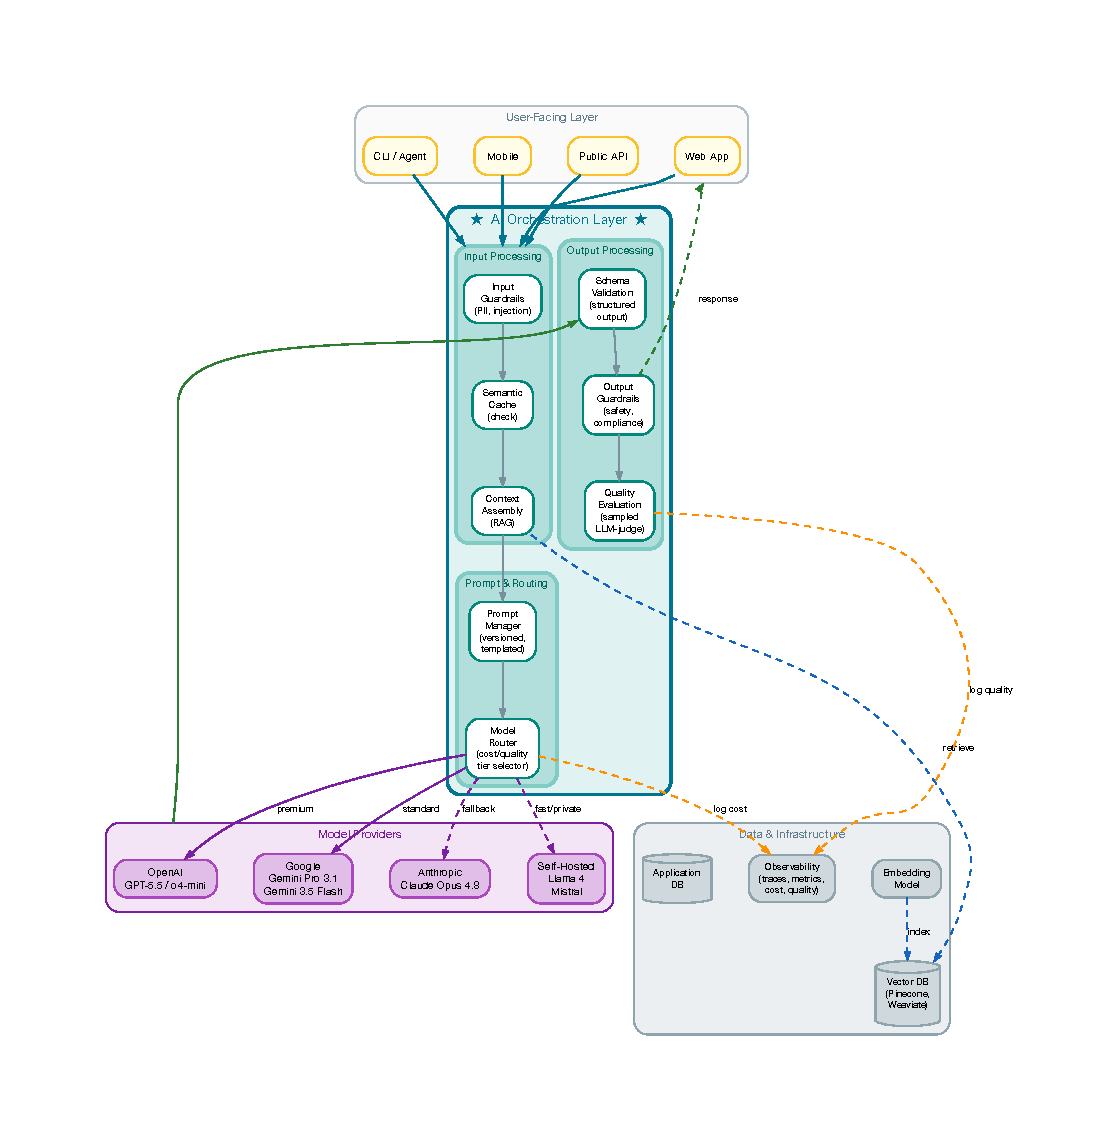
\includegraphics[width=\textwidth]{diagrams/compiled/ch01/new-software-stack.pdf}
\caption{The modern software stack with the AI orchestration layer}
\label{fig:new-stack}
\end{figure}

The AI orchestration layer includes:

\begin{itemize}[leftmargin=*]
  \item \textbf{Prompt management}: Versioning, templating, and A/B testing of prompts
  \item \textbf{Context assembly}: Retrieving and formatting relevant information (RAG)
  \item \textbf{Model routing}: Selecting the right model for each request based on cost, latency, and quality requirements
  \item \textbf{Output validation}: Parsing, validating, and sanitizing model outputs
  \item \textbf{Evaluation}: Measuring output quality in production
  \item \textbf{Guardrails}: Safety filters, PII detection, content policy enforcement
  \item \textbf{Caching}: Semantic caching to reduce cost and latency
  \item \textbf{Fallback logic}: Graceful degradation when model calls fail or return low-quality results
\end{itemize}

Each of these components requires careful engineering. Together, they constitute a new discipline that this book calls \term{AI engineering}---the practice of building reliable, scalable, and maintainable systems that incorporate language models.

\section{Five Problems That Changed Overnight}

To make the paradigm shift concrete, consider five engineering tasks that every software team does---and how LLMs have fundamentally altered the approach to each. Figure~\ref{fig:five-problems} shows the before and after.

\begin{figure}[htbp]
\centering
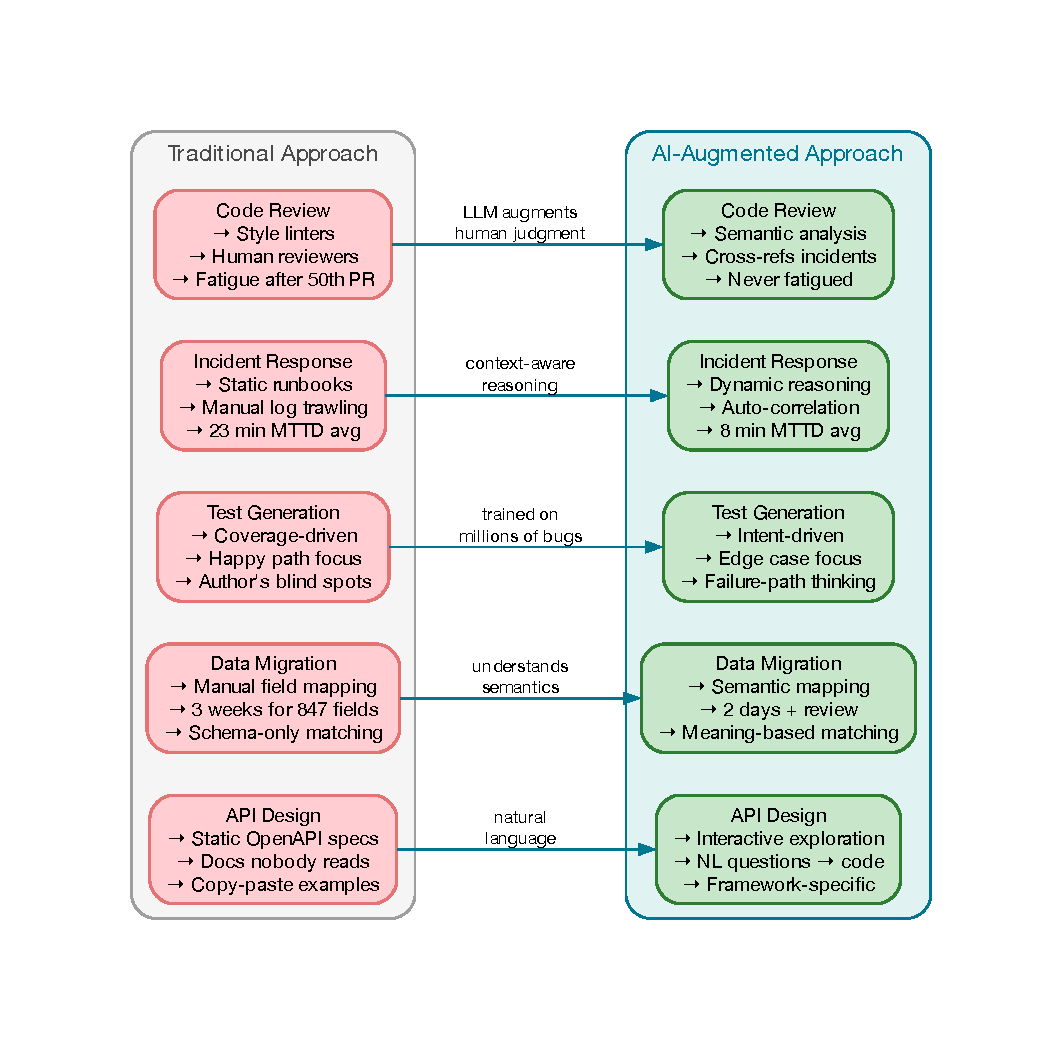
\includegraphics[width=\textwidth]{diagrams/compiled/ch01/five-problems.pdf}
\caption{Five engineering tasks that LLMs have fundamentally transformed: from manual, rule-based approaches to semantic, AI-augmented workflows}
\label{fig:five-problems}
\end{figure}

\subsection{Code Review: From Stylistic Nitpicks to Semantic Analysis}

A traditional linter catches formatting errors. A human reviewer catches logic errors. An LLM-powered code reviewer can do something neither can: reason about \emph{intent}. At multiple fintech companies, LLM-augmented code review systems now run on every PR to payments services, cross-referencing diffs against recent incidents, architecture docs, and compliance requirements. They catch $\sim$30\% of issues that human reviewers miss---primarily missing error handling, race conditions, and PCI compliance gaps.

The key insight is not that LLMs can review code---it's that they review code \emph{differently} than humans. They don't get fatigued after the 50th PR of the day. They don't have the ``LGTM after glancing at it for 30 seconds'' failure mode. And they can cross-reference every PR against the last six months of incidents, which no human reviewer does consistently.

\subsection{Incident Response: From Runbooks to Reasoning}

When a production service goes down at 3 AM, an on-call engineer follows a runbook. But runbooks are static, and incidents are dynamic. LLM-augmented incident response systems gather context automatically---metrics from Prometheus, recent deploys, similar past incidents from the incident database, error logs from the last 15 minutes---and reason about the specific combination of symptoms. One B2B SaaS company reported reducing mean-time-to-diagnosis from 23 minutes to 8 minutes. Crucially, these systems \emph{recommend} actions but do not take them autonomously---the human engineer remains in the loop for all mitigation steps.

\subsection{Test Generation: From Coverage Gaps to Intent Coverage}

Traditional test generators produce assertions based on existing behavior. LLMs generate tests based on what the code \emph{should} do---including edge cases the author forgot:

\begin{lstlisting}[language=Python, caption={Intent-driven test generation: LLMs probe failure modes the author didn't consider}]
# What a coverage tool generates: exercises lines
def test_process_payment_basic():
    result = process_payment(amount=100, currency="USD")
    assert result.status == "success"

# What an LLM generates: probes intent and failure paths
def test_process_payment_idempotency():
    """Same idempotency key should not charge twice."""
    key = "idem_abc123"
    r1 = process_payment(100, "USD", idempotency_key=key)
    r2 = process_payment(100, "USD", idempotency_key=key)
    assert r1.charge_id == r2.charge_id  # Not double-charged

def test_process_payment_timeout_during_bank_call():
    """Network timeout mid-charge must not leave orphaned holds."""
    with mock_timeout(target="bank_api.charge", after_ms=500):
        with pytest.raises(PaymentTimeoutError):
            process_payment(amount=100, currency="USD")
    assert get_pending_holds(test_account) == []
\end{lstlisting}

The LLM-generated tests are better not because the LLM is smarter than the engineer, but because it isn't suffering from the same cognitive biases. The author of \code{process\_payment} naturally thinks about the happy path. The LLM, having been trained on millions of bug reports and test suites, thinks about the failure paths.

\subsection{Data Migration: From Schema Scripts to Semantic Mapping}

Perhaps the most surprising application: LLMs can reason about the \emph{meaning} of data, not just its structure. A team migrating from a legacy CRM to a modern system used an LLM to map 847 custom fields---a task that would have taken weeks of manual analysis. The model correctly mapped 91\% of fields on the first pass by understanding domain context (e.g., recognizing that \code{cust\_npi} is a National Provider Identifier and maps to the \code{provider.npi} field). Human review corrected the remaining 9\%, reducing the project timeline from 3 weeks to 2 days.

\subsection{API Design: From Documentation to Interactive Contracts}

LLMs are changing how APIs are designed and consumed. Instead of writing OpenAPI specs that nobody reads, teams embed the spec in an LLM's context and let developers ask questions in natural language: ``How do I paginate through all transactions for a given customer?'' The model generates working code, complete with error handling and pagination logic, customized to the developer's language and framework.

\begin{keytakeaway}
The common thread across all five examples is the same: LLMs don't replace engineering judgment---they \emph{accelerate} it. They handle the tedious parts (reading 847 field descriptions, scanning 50 PRs, correlating metrics at 3 AM) so that engineers can focus on the parts that require genuine expertise (architectural decisions, security implications, business logic correctness). The danger is not that LLMs will replace engineers. The danger is that engineers who refuse to use LLMs will be replaced by engineers who do.
\end{keytakeaway}



\section{What This Book Is and Isn't}

This book is \emph{not} an introduction to machine learning. We assume you know what a neural network is, what gradient descent does, and why GPUs are used for training. If you need a refresher, Appendix~B lists excellent resources.

This book \emph{is} a systems engineering guide for the AI era. We treat LLMs the way \emph{Software Engineering at Google}~\cite{winters2020swe} treats distributed systems: as powerful but complex components that require disciplined engineering practices to use effectively at scale.

We focus on:

\begin{enumerate}[leftmargin=*]
  \item \textbf{How things actually work}: Not marketing descriptions, but the real architectures, trade-offs, and failure modes
  \item \textbf{Proven patterns}: Architecture patterns that have been validated in production at companies like Google, Stripe, GitHub, and LinkedIn
  \item \textbf{Practical guidance}: Concrete code examples, configuration templates, and decision frameworks you can apply immediately
  \item \textbf{Engineering discipline}: Testing strategies, monitoring approaches, and operational practices specific to AI systems
\end{enumerate}

\section{How This Book Is Organized}

The book follows the natural progression of an engineer's journey with LLMs:

\textbf{Part I (Chapters 1--4)} builds your foundational understanding of how LLMs are created. You'll learn about pre-training, post-training, and fine-tuning---not from a researcher's perspective, but from an engineer's. The question is not ``how does backpropagation work?'' but ``what are the infrastructure requirements for training a 70B parameter model, and what are the failure modes?''

\textbf{Part II (Chapters 5--8)} covers building production systems with LLMs. Architecture patterns, enterprise case studies, data engineering, and the critically underserved topic of evaluation and testing for AI systems.

\textbf{Part III (Chapters 9--11)} examines how AI is changing software engineering itself---the tools, the team structures, and the operational practices.

\textbf{Part IV (Chapters 12--15)} looks forward to the era of AI agents and autonomous systems, with deep technical guidance on building agents that actually work in production.

\textbf{Part V (Chapters 16--17)} provides interview preparation material with over 90 carefully crafted questions in Python programming and systems design, drawn from real interview loops at top AI companies.

\begin{keytakeaway}
Software engineering in the age of AI is not about replacing engineering with AI. It's about \emph{extending} the discipline of engineering to encompass a new class of computational primitives. The engineers who thrive will be those who combine deep software engineering expertise with a practical understanding of how AI systems work, fail, and can be made reliable.
\end{keytakeaway}
